\section{Modeling A Preferential Pathway}

To investigate the role a land drain type preferential pathway may have on a VI site, we extend the VI model presented in Chapter \ref{chp:method}.
By adding a gravel sub-base layer underneath the foundation slab and a preferential pathway to this model, we develop a VI model scenario that is similar to the ASU house.\par

Here we assume the gravel sub-base layer is \SI{30}{\centi\metre} thick and extends from the edges of the foundation slab.
While the exact thickness of the gravel sub-base layer at the ASU house is not known, it was estimated to be roughly that thick.
The soil surrounding the house is assumed to be homogenous sandy clay.
This is based on a description of the soil, and was chosen as the most appropriate choice is some modeling work  by \citeauthor{guo_vapor_2015}\cite{guo_vapor_2015}, one of the researchers at the ASU house.\par

The gravel sub-base, unlike the rest of the soil, is going to be relatively dry; it is covered by the foundation slab, so no rain infiltration will occur and due to the coarseness of the gravel, no moisture will be drawn up by capillary force.
Nonetheless, some van Genuchten parameters for the gravel are necessary to solve the model.
Additionally, based on the site description, we will assume that the surrounding soil is sandy clay, a , one of the researchers at the ASU house.
Table \ref{tbl:soils} has the van Genuchten parameters used to model these.\par

\begin{figure}[hbt!]
  \centering
  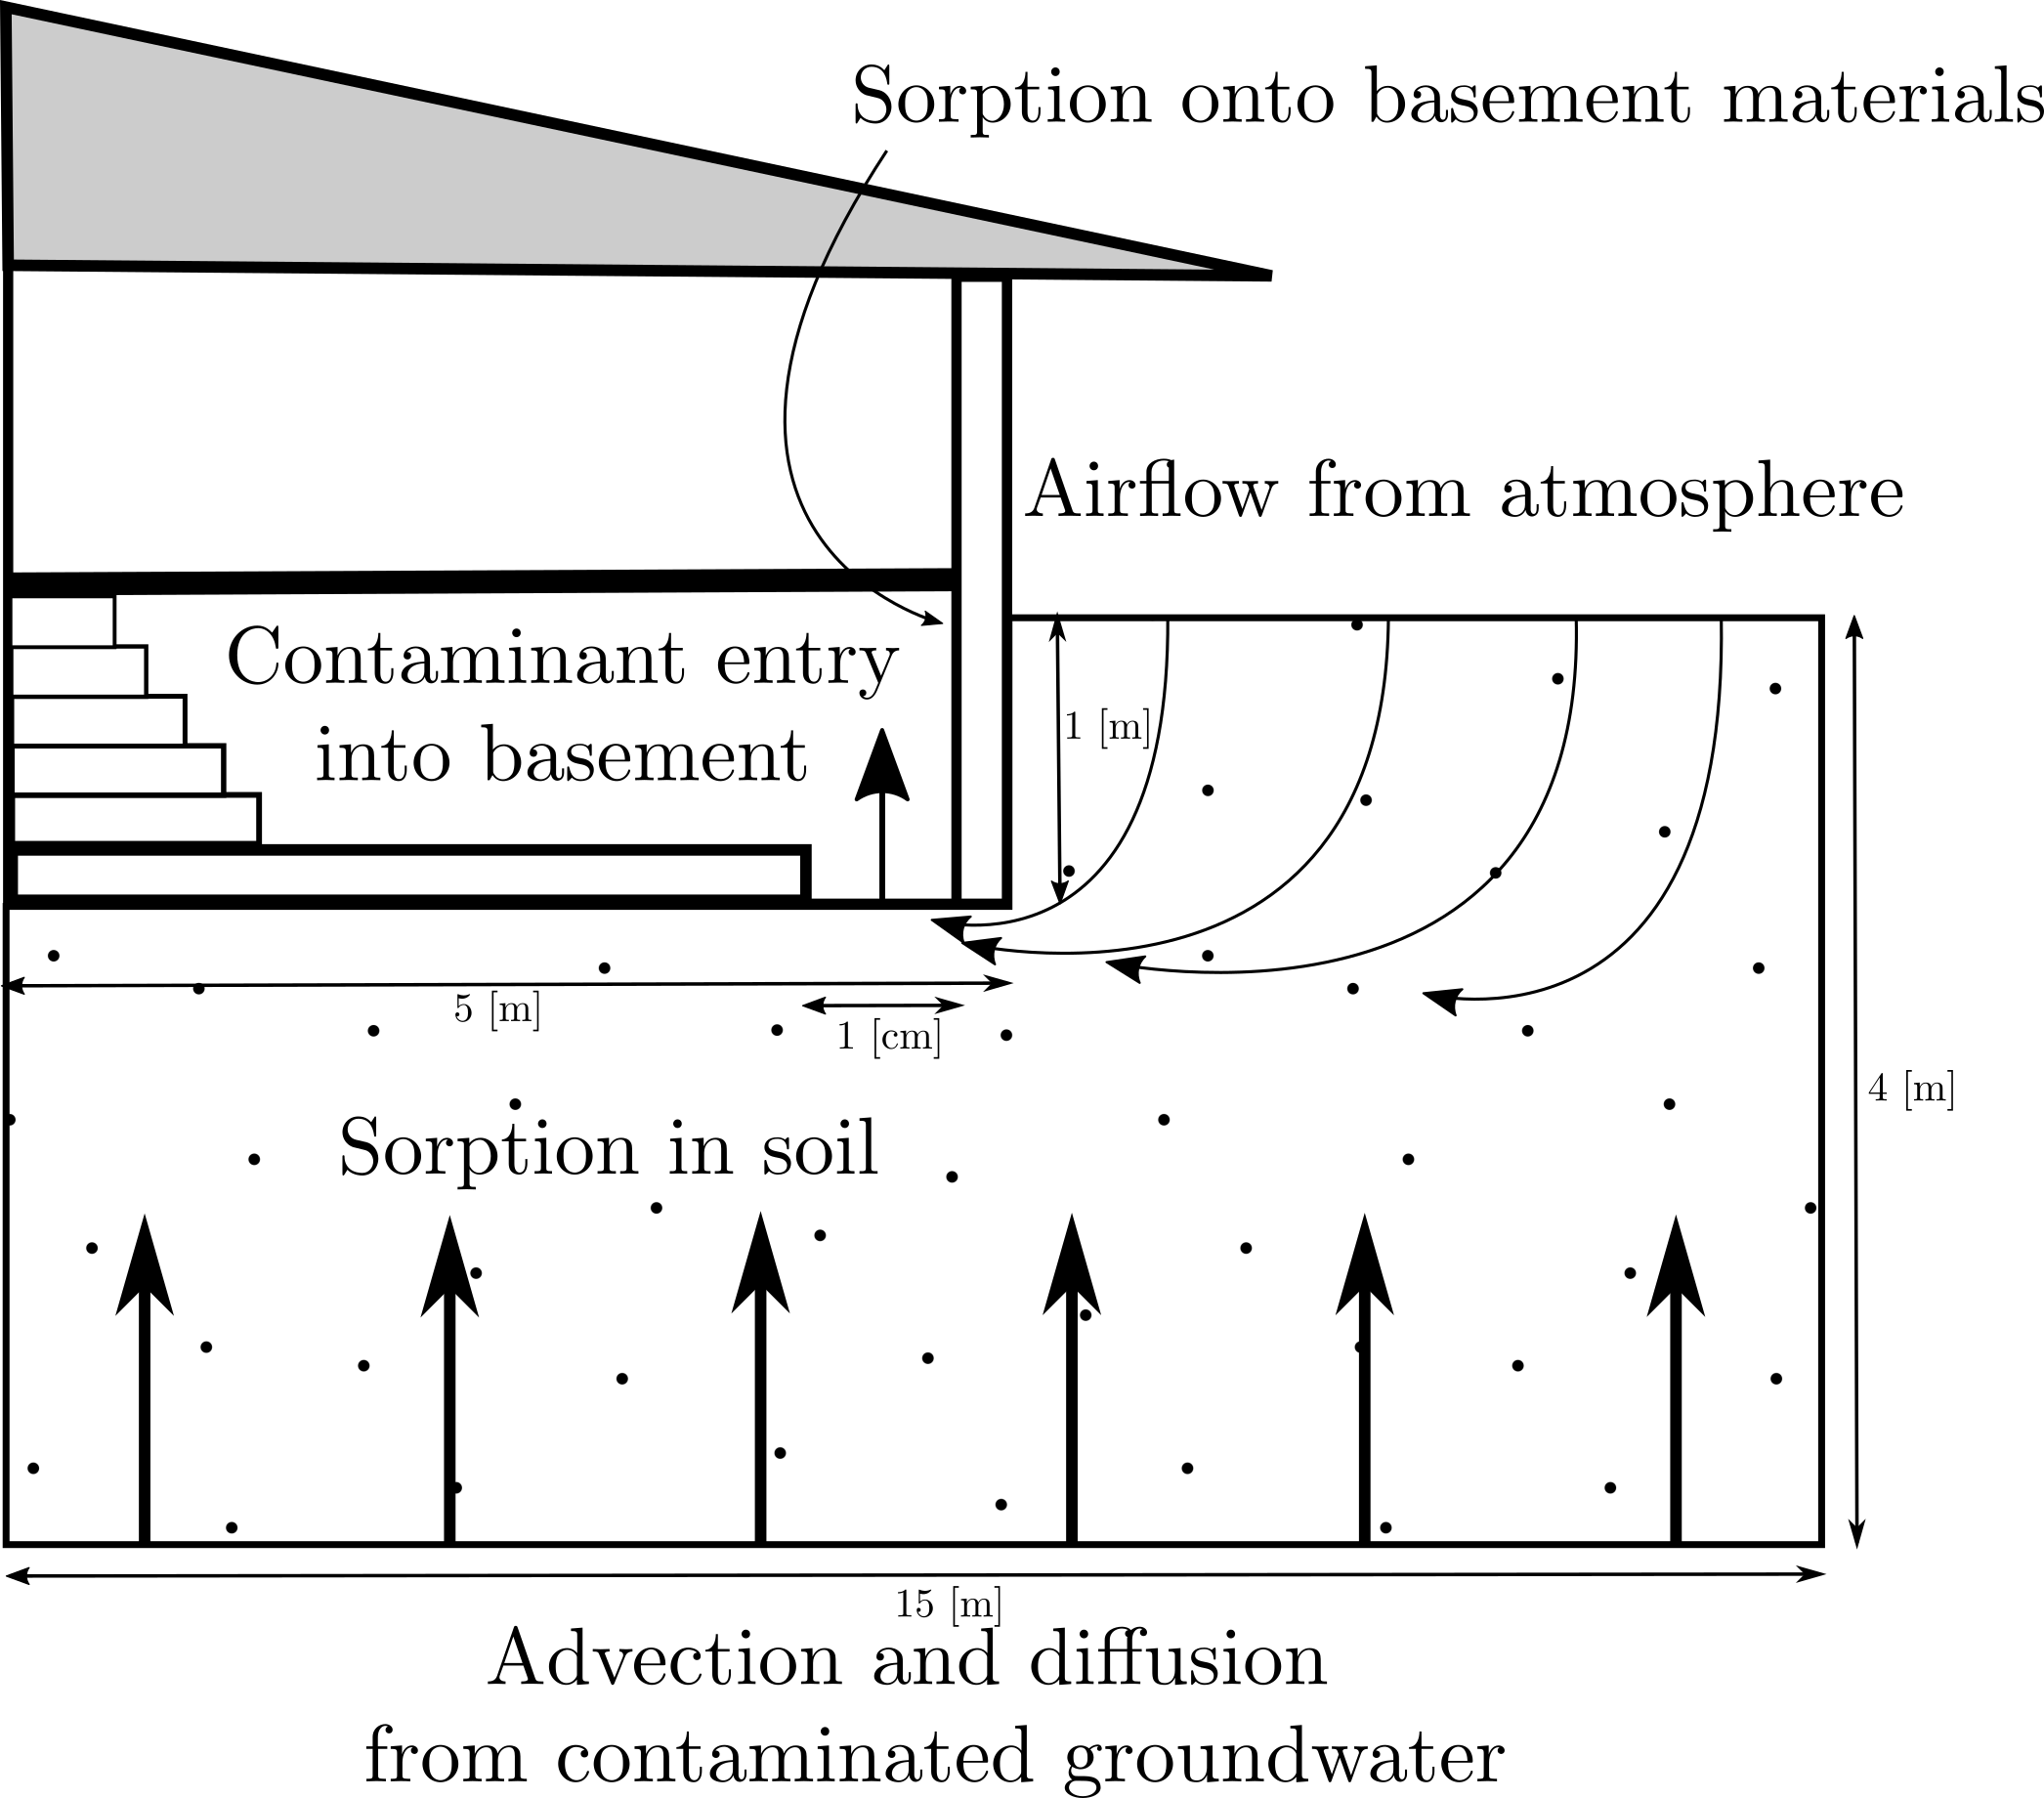
\includegraphics[width=0.75\textwidth]{model.png}
  \caption{The modeled preferential pathway VI scenario.}
  \label{fig:model_preferential_pathway}
\end{figure}

Based on the description of the land drain preferential pathway at the ASU site, we will model a preferential pathway as \SI{10}{\centi\metre} diameter pipe that exits at the interface between the soil and gravel sub-base layer; placing it near the foundation crack - similar to the ASU house\cite{guo_identification_2015}.
Figure \ref{fig:model_preferential_pathway} shows the described scenario.\par


\subsection{Geometry And Mesh}

Explicitly modeling the entire preferential pathway in detail would requires a significant number of elements and at little gain; contaminant vapor transport in the far corners of the model are not of great interest.
To save computational resources only the exit of the pipe is modeled as a \SI{10}{\centi\metre} diameter circle.\par

The existence of the preferential pathway pipe circle, only one plane of symmetry exists instead of two, and half of the model geometry has to be explicitly constructed instead of just a quarter like in Chapter \ref{chp:method}.\par

The meshing of the model follows the steps detailed in Chapter \ref{chp:method}, with the exception that a boundary layer mesh generated on the preferential pathway circle; a similar initial mesh is generated with subsequent adaptive mesh refinement.
Figure \ref{fig:model_meshed} shows the resulting meshed geometry.\par

% TODO Add mesh information in the description.
% TODO Get an image of the adapted mesh, or is this it?
\begin{figure}[htb!]
  \centering
  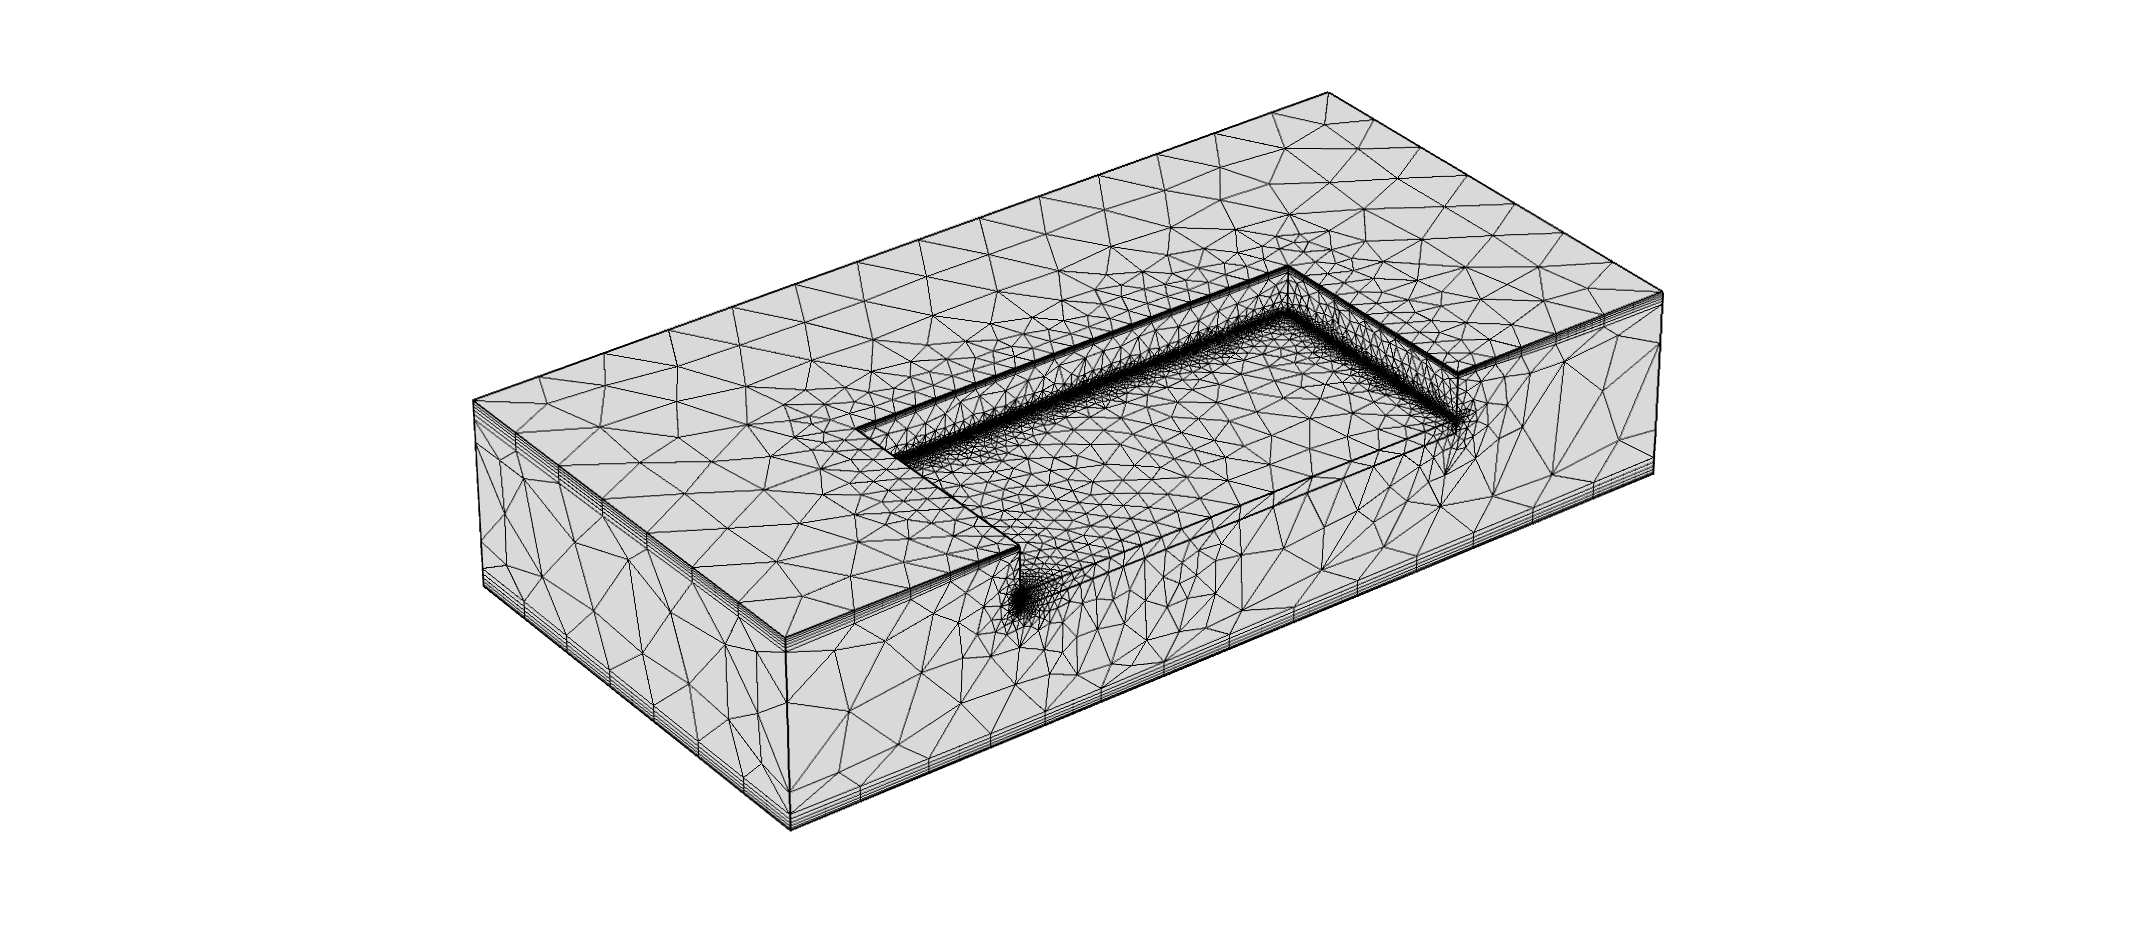
\includegraphics[width=0.75\textwidth]{model_meshed.png}
  \caption{Meshed geometry of the preferential pathway model. Notice the gravel sub-base layer and the preferential pathway exit.}
  \label{fig:model_meshed}
\end{figure}

\subsection{Physics And Boundary Conditions}

In this model, we use the same governing equations introduced in Chapter \ref{chp:method}, but are included here for completeness.
However, to simulate the preferential pathway, we will need to supply two new boundary conditions  - one for the airflow in the soil governed by Darcy's Law, and another for the soil contaminant transport, which are discussed in their respective section below.

\subsubsection{Indoor Environment}

The indoor environment is modeled using:
\begin{align*}
    V_\mathrm{bldg}\frac{\partial c_\mathrm{in}}{\partial t} &= n_\mathrm{ck} - V_\mathrm{bldg} A_e c_\mathrm{in} \\
    n_\mathrm{ck} &= \int_{A_\mathrm{ck}} j_\mathrm{ck} dA \\
    j_{ck} &= \begin{cases}
      u_{ck} c_g - \frac{D_\mathrm{air}}{L_\mathrm{slab}} (c_{in} - c_g) & u_{ck} \geq 0 \\
      u_{ck} c_{in} - \frac{D_\mathrm{air}}{L_\mathrm{slab}} (c_{in} - c_g) & u_{ck} < 0
  \end{cases}
\end{align*}
$c_\mathrm{in}$ [\si{\mol\per\metre\cubed}] is the indoor contaminant concentration;
$n_\mathrm{ck}$ [\si{\mol\per\second}] is the contaminant entry rate into the building via the foundation crack;
$A_\mathrm{ck}$ [\si{\metre\squared}] is the foundation crack boundary area;
$A_e = \SI{0.5}{\per\hour}$ is the air exchange rate;
$V_\mathrm{bldg} = \SI{300}{\metre\cubed}$ is the volume of the house basement.
$D_\mathrm{air} = \SI{7.2e-6}{\metre\squared\per\second}$ is the diffusion coefficient of TCE in air;
$u_{ck}$ [\si{\metre\per\second}] is the airflow velocity through the foundation crack;
$L_\mathrm{slab} = \SI{15}{\centi\metre}$ is the thickness of the foundation slab;
and $c_g$ [\si{\mol\per\metre\cubed}] is the contaminant gas-phase concentration at the foundation crack boundary.\par

\subsubsection{Soil Moisture}

Soil moisture content is determined using van Genuchten's retention model.
We use two "soil" types in this model - gravel and sandy clay; their parameters and constants are shown in Table \ref{tbl:soils} in the appendix.
\begin{align*}
  \mathrm{Se} &=
    \begin{cases}
      \frac{1}{(1 + (\alpha |h|)^n)^m} & \quad\quad\quad\quad\quad\quad h < 0 \\
    1 & \quad\quad\quad\quad\quad\quad h \geq 0
    \end{cases}\\
  \theta_w &=
    \begin{cases}
      \theta_r + \mathrm{Se}(\theta_t - \theta_r) & \quad\quad\quad\quad h < 0 \\
      \theta_t & \quad\quad\quad\quad h \geq 0
    \end{cases}\\
    k_r &= \begin{cases}
        \mathrm{Se}^l \big[ 1 - \big( 1 - \mathrm{Se}^\frac{1}{m} \big) \big]^2 & \quad\quad h < 0 \\
        0 & \quad\quad h \geq 0
      \end{cases}\\
    \theta_g &= \theta_t - \theta_w
\end{align*}
$h$ [\si{\metre}] is the elevation above the groundwater interface;
$\mathrm{Se}$ is the saturation;
$\alpha$, $m$, $n=\frac{1}{1-m}$, $l=0.5$ are the van Genuchten parameters;
$\theta_w$ is the water filled porosity;
$\theta_g$ is the gas filled pororsity;
$\theta_t$ is the soil porosity;
$\theta_r$ is the residual moisture content.
and $k_r$ is the relative permeability for water;

\subsubsection{Soil Airflow}

Airflow is modeled using our modified Darcy's Law expression.
\begin{equation*}
  \frac{\partial}{\partial t} (\rho \theta_g) + \nabla \cdot \rho \Big( -\frac{(1-k_r) \kappa}{\mu} \nabla p \Big) = 0
\end{equation*}
$\vec{u}$ [\si{\m\per\second}] is the airflow velocity vector;
$\kappa$ [\si{\metre\squared}] is the permeability of the porous medium;
$\mu$ [\si{\pascal\second}] is the dynamic viscosity of the fluid;
$\nabla p$ [\si{\pascal\per\metre}] is the pressure gradient;
$\theta_g$ is the gas-filled porosity of the soil;
$\rho = \SI{1.225}{\kilogram\per\metre\cubed}$ is the density of air;
and $\mu = \SI{18.5e-6}{\pascal\second}$ is the dynamic viscosity of air.\par

\paragraph{Boundary conditions}

Since the preferential pathway is assumed to be an open pipe, we assume it acts like a pressure gauge, just like the atmosphere, and is at the reference ambient atmospheric pressure.
\begin{align*}
    &\text{Ground surface} &p = \SI{0}{\pascal} \\
    &\text{Preferential pathway} &p = \SI{0}{\pascal} \\
    &\text{Foundation crack} &p = p_\mathrm{in/out} \; \si{\pascal} \\
    &\text{Remaining} &-\vec{n}\cdot\rho\vec{u} = 0
\end{align*}
$p_\mathrm{in/out}$ is not specified here as we will parametrically choose values for it.\par

\subsubsection{Soil Contaminant Transport}

The contaminant transport in the soil is governed by:
\begin{equation*}
  (\theta_w + \theta_g K_H) \frac{\partial c_w}{\partial t} = \nabla \cdot (D_\mathrm{eff} \nabla c_w) - K_H \vec{u}_g \cdot \nabla c_w
\end{equation*}
$c_w$ and $c_g$ [\si{\mol\per\metre\cubed}] are the contaminant concentrations in water and gas respectively;
$K_H = 0.402$ is the dimensionless Henry's Law constant for TCE at \SI{20}{\degreeCelsius};
$\vec{u}_g$ [\si{\metre\per\second}] is the Darcy's velocity field;
and $D_\mathrm{eff}$ [\si{\metre\squared\per\second}] is the effective diffusivity of the contaminant according to Millington-Quirks model:
\begin{equation*}
  D_\mathrm{eff} = \Big(D_w \frac{\theta_w^{\frac{10}{3}}}{\theta_t^2} + D_g \frac{\theta_g^{\frac{10}{3}}}{\theta_t^2} K_H\Big)
\end{equation*}
$D_w = \SI{1.02e-9}{\metre\squared\per\second}$ and $D_g = \SI{6.87e-6}{\metre\squared\per\second}$ are the diffusion coefficient of TCE in water and air respectively;

\paragraph{Boundary conditions}

The air in the pipe is assumed to be contaminated with TCE at a vapor concentration equal to the vapor in equilibrium with the groundwater source contaminant concentration.
This assumption is based on contaminant samples taken from a manhole near the ASU house\cite{guo_vapor_2015} which demonstrated that contaminant vapor concentrations in the nearby sewer were on similar magnitude as near the contaminated groundwater source.
\begin{align*}
  &\text{Atmosphere} & c_w = \SI{0}{\mol\per\metre\cubed} \\
  &\text{Groundwater} & c_w = c_{gw} \; \si{\mol\per\metre\cubed} \\
  &\text{Preferential pathway} & c_g = c_{gw} K_H \; \si{\mol\per\metre\cubed} \\
  &\text{Foundation crack} & -\vec{n} \cdot \vec{N} = \frac{-j_{ck}}{K_H} \; \si{\mol\per\metre\squared\per\second}\\
  &\text{All other} & -\vec{n} \cdot \vec{N} = \SI{0}{\mol\per\metre\squared\per\second}
\end{align*}
Note that we are neglecting any sorption in the soil, i.e. the sorption partitioning coefficient $K_p = \SI{0}{\metre\cubed\per\kilo\gram}$.
We will likewise normalize all concentrations to the source concentration $c_{gw}$, and any arbitrary value can be assigned.\par
